\documentclass[a4paper,12pt]{report}

\usepackage[utf8]{inputenc}
\usepackage{graphicx}
\usepackage{hyperref}
\usepackage{multirow}
\usepackage{multicol}
\usepackage{amsmath,amsfonts,amssymb,amsthm,mathrsfs,mathtools}
\usepackage{cancel}
\usepackage{bm}
\usepackage[table,svgnames, dvipsnames]{xcolor}
\usepackage{fancyhdr}
    \setlength{\headheight}{14.5pt}
\usepackage{minted}
% \usemintedstyle{borland}
% \usepackage[minted]{tcolorbox}
%     \newtcblisting{mylisting}{listing only,listing engine=minted, minted language=py, minted style=borland,colback=gray!20}
\usepackage{subcaption}
\usepackage{booktabs}
\usepackage{pgfgantt,pgfplotstable,pgfplots}
\usepackage{tikz-uml}
\usepackage{csvsimple}
\usepackage{makecell}
\usepackage{xcolor}
\usepackage{framed}
\usepackage{enumerate}
\usepackage{pdflscape}
% \usepackage{siunitx}
\usepackage{units}
\usepackage[T1]{fontenc}
\usepackage{libertine}
\usepackage{sectsty}
    \allsectionsfont{\biolinum}
    
% --- Let us remove soul to make sure we don't use \st anywhere...    
% \usepackage{soul}

\definecolor{codegreen}{rgb}{0,0.6,0}
\definecolor{codegray}{rgb}{0.5,0.5,0.5}
\definecolor{codepurple}{rgb}{0.58,0,0.82}
\definecolor{backcolour}{rgb}{0.95,0.95,0.92}
\definecolor{airforceblue}{rgb}{0.36, 0.54, 0.66}
\definecolor{rosequartz}{rgb}{0.96, 0.75, 0.76}

\pgfplotsset{compat=1.18}

% \lstdefinestyle{mystyle}{
% 	backgroundcolor=\color{backcolour},   
%     commentstyle=\color{codegreen},
%     keywordstyle=\color{magenta},
%     numberstyle=\tiny\color{codegray},
%     stringstyle=\color{codepurple},
%     emph={mass,arm_length,K_v,voltage_max,voltage_min,prop_diameter_in},  % Custom highlighting
%     emphstyle=\color{codepurple},  % Custom highlighting style
%     basicstyle=\ttfamily\footnotesize,
%     breakatwhitespace=false,         
%     breaklines=true,                 
%     captionpos=b,                    
%     keepspaces=true,                 
%     numbers=left,                    
%     numbersep=5pt,                  
%     showspaces=false,                
%     showstringspaces=false,
%     showtabs=false,                  
%     tabsize=2
% }

% \lstset{style=mystyle}

% \numberwithin{equation}{section}
% \synctex=1

\setlength{\parindent}{0pt}  
\setlength{\parskip}{8pt}

\hypersetup{
    unicode=false,          % non-Latin characters in Acrobat’s bookmarks
    pdftoolbar=true,        % show Acrobat’s toolbar
    pdfmenubar=true,        % show Acrobat’s menu
    pdffitwindow=false,     % window fit to page when opened
    pdfstartview={FitH},    % fits the width of the page to the window
    pdfnewwindow=true,      % links in new PDF window
    colorlinks=true,        % false: boxed links; true: colored links
    linkcolor=red,          % color of internal links (change box color with linkbordercolor)
    citecolor=blue,         % color of links to bibliography
    filecolor=magenta,      % color of file links
    urlcolor=cyan           % color of external links
}
\urlstyle{same}

\usepackage{geometry}
% \linespread{1.5}
\geometry{
	a4paper,
	left=25mm,
	right=25mm,
	top=25mm,
	bottom=25mm,
}

\pagestyle{fancy}
\fancyhf{}
\rhead{\thepage}

% Custom commands
% \newcommand{\commentPS}[1]{{\color{green!70!black}#1}}
% \newcommand{\commentRM}[1]{{\color{red!70!black}#1}}
% ---- Let us deactivate all comments... ---
\newcommand{\commentPS}[1]{}
\newcommand{\commentRM}[1]{}
% ------------------------------------------


% --- Definitions -------------------
\newcommand{\R}{{\rm I\!R}}
\newcommand{\E}{{\rm I\!E}}
\newcommand{\N}{{\rm I\!N}}
\newcommand{\Hamilton}{{\rm I\!H}}
\newcommand{\q}{\mathfrak{q}}
\newcommand{\p}{\mathfrak{p}}
\newcommand{\smallmat}[1]{\left[ \begin{smallmatrix}#1 \end{smallmatrix} \right]}
\newcommand\tab[1][1cm]{\hspace*{#1}}
\newcommand{\minimise}{\operatorname*{Minimise}}
\newcommand{\fnstt}[1]{{\texttt{\footnotesize #1}}}
\newcommand{\ttop}{{\scalebox{.75}{$\scriptscriptstyle \top$}}}
\newcommand{\Var}{\operatorname{Var}}
\newcommand{\Cov}{\operatorname{Cov}}
\newcommand{\dfn}{\mathrel{\mathop:}=}
\newcommand{\NN}{\mathcal{N}}
\newcommand{\dd}{\mathrm{d}}

% --- Acronyms ---
\usepackage{acronym}


\begin{document}
    \begin{titlepage}
    \thispagestyle{empty}
    \begin{center}
        {Queen's University Belfast}\\[0.4cm]
        {School of Electronics, Electrical Engineering and Computer Science}\\[1cm]
        \hbox{}\hfill
        \begin{minipage}[t]{\textwidth}
        \begin{center}
            
\includegraphics[width=0.5\textwidth]{figures/logo.jpg}
        \end{center}
        \end{minipage}
        \hfill\hbox{}
        \\[3cm]
        {\large BSc (Hons) Final Year Project Report\\[0.3cm]}
        {\LARGE \bfseries \biolinum GPU-Accelerated Solution for the Black-Scholes equation \\[3cm]}
        {\large Chelsea De Marseilla, 40329124}\\[0.4cm]
        {\large \today}
    \end{center}
    \vspace*{\fill}
    \begin{minipage}[t]{0.48\textwidth}
        {Supervisor:}\\[0.3cm]
        {\large Dr P. Sopasakis}\\[0.1cm]
        School of EEECS
    \end{minipage}
    \hfill
\end{titlepage}


\clearpage
\setcounter{page}{0}

\newpage
\pagenumbering{roman}
\chapter*{Abstract}
abstract

\pagebreak
\tableofcontents
\pagebreak



\pagenumbering{arabic}

\chapter{Problem statement} \label{sec:problem_statement}
% ~2 PAGES
% Objectives (hi-level, specific), blah
% O1. Understand the intimate relationship between the BSE and the heat equation and implemnet a solver for the BSE based on the heat equation (the motivation is that we will then be able to use widely available solvers for the heat equation to solve the BSE) + verify correctness
% O2. Use the GBM to perform MC simulations and evaluate the behaviour of BS-based option pricing in realistic conditions
% O3. GPU parallelisation of numerical methods and measurement of speed-up (what exactly will be parallelised: BOTH numerical mehtods for PDEs AND GBM)

\section{Introduction and Motivation}
The Black-Scholes equation is a fundamental partial differential equation used in financial mathematics to estimate the theoretical fair value of financial derivatives, particularly European-style options. Through this equation, the evolution of option prices can be modelled by taking into account multiple factors such as the price of the underlying asset (S), the time to expiration (T), volatility ($\sigma$) and the risk-free rate (r).

The complex nature of partial differential equations (PDEs) presents significant challenges in obtaining general solutions. While an analytical solution to the Black-Scholes equation exists, it is only applicable to a limited class of financial derivatives, particularly European-style options. For more complex options, such as American options or exotic options, closed-form analytical solutions either do not exist or become extremely difficult to obtain. This limitation introduces the need for numerical methods to approximate solutions for such equations. However, the ability to solve PDEs numerically comes with a trade-off, as the computational demands can be significant and time-consuming. This is particularly true when dealing with Monte Carlo simulations for option pricing which require large sampling sizes to achieve accurate results.

Recent advances in parallel computing has opened up new possibilities for accelerating the computations required for numerical methods. By leveraging the power of Graphics Processing Units (GPUs), it becomes possible to achieve significant speed-ups in solving PDEs, making it feasible to tackle more complex problems that were previously computationally intractable.

This project proposes a GPU-accelerated solution for the Black-Scholes equation by exploiting the mathematical equivalence\cite{wilmott_1995_mathematics} between the one-dimensional heat equation and the Black-Scholes equation. Although separate solvers were developed for each equation, the transformation between the two provides a theoretical foundation for applying similar numerical methods, thereby enabling efficient approximation of solutions for option pricing. Finite difference methods were used to solve the PDEs, and Monte Carlo simulations were employed to price options by modelling the stochastic behaviour of the underlying asset.

Alongside parallelisation on the GPU machine, this project also involves the development of an open-source Python library for solving partial differential equations, distributed as a PyPI package. This library will provide users with the ability to define and solve various PDEs with minimal effort.

\section{Objectives}
The objectives of this project are as follows:
\begin{enumerate}
    \item Understand the intimate relationship between the heat equation and the Black-Scholes equation
    \item Implement solvers for both the Black-Scholes equation and the heat equation using finite difference schemes
    \item Verify the correctness of the solvers by comparing the numerical solutions with each other and with analytical solutions
    \item Develop a Python library for solving PDEs, which will be distributed as a PyPI package
    \item Use the Geometric Brownian Motion (GBM) model to perform Monte Carlo simulations for Black-Scholes based option pricing in realistic conditions
    \item Implement GPU parallelisation of the numerical methods, particularly the computationally intensive parts of the code, to achieve significant speed-ups
    \item Measure the performance of the GPU-accelerated solution and compare it with the CPU-based solution
\end{enumerate}

% ~2 PAGES
% Objectives (hi-level, specific), blah
% O1. Understand the intimate relationship between the BSE and the heat equation and implemnet a solver for the BSE based on the heat equation (the motivation is that we will then be able to use widely available solvers for the heat equation to solve the BSE) + verify correctness
% O2. Use the GBM to perform MC simulations and evaluate the behaviour of BS-based option pricing in realistic conditions
% O3. GPU parallelisation of numerical methods and measurement of speed-up (what exactly will be parallelised: BOTH numerical mehtods for PDEs AND GBM)


\chapter{Derivatives and Option Pricing: Literature Review}
% BACKGROUND
\label{sec:literature}
\section{Introduction to Derivatives and Option Pricing}
Over the years, derivatives trading has emerged as a fundamental component of modern finance,
evolving into a widespread practice across global financial markets. This shift in market dynamics
introduces a challenge in determining the fair value (price) of derivative products, and in turn,
ensure a balanced outcome for both the buyer and the seller.

A \textit{financial derivative} is primarily known as a financial instrument whose value depends on the
values of more basic underlying variables \cite{hull_2021_options}. These derivatives come in many forms,
with examples such as \textit{futures contracts, options, and swaps}, each typically derived from the prices of
the traded assets. An \textit{option} is a derivative security which gives the holder the right (but not the obligation) 
to purchase or sell an underlying asset at a certain price by a predetermined time. The holder may decide to buy or sell
the purchased option based on whether the conditions are favourable to them; if not, they may choose to let the option expire worthless. 
Knowing this definition of an option, it can be divided into two different types: \textit{call} or \textit{put} options. A simple \textit{call} option 
is a contract that gives the holder the right to buy an asset at an agreed price by a specified time. A simple \textit{put} 
option, on the other hand, is a contract that gives the holder the right to sell an asset at an agreed price by a specified time.
The price at which the option can be exercised is known as the \textit{exercise} or \textit{strike} price, and the date on which
the option needs to be exercised by is the \textit{expiration} date or \textit{maturity}. Typically, an option is exercised only at
its expiration time\textemdash these are known as \textit{European} options. Otherwise, it is considered an \textit{American} option
which allows the holder to exercise the option prior to its expiration.
\subsubsection{Example of a Call Option} 
Suppose a European call option for 100 shares of NVIDIA stock is created with a strike price of \$100 and an expiration date in one month. 
The price of an option for each individual share of the stock is \$8, making the initial investment a total of \$800. If, in one month's time,
the stock falls below the strike price (\$100), it would be unfavourable for the holder to exercise the option, as it would then be worthless.
The holder then loses their initial investment of \$800. In the favourable case where the stock rises to a price of \$120 at expiry, the option
will be exercised. Here, the holder buys 100 shares of the stock at the agreed strike price (\$100). Selling their stocks immediately would 
lead to a gain of \$2000, and a net profit of \$1200 (taking into account the initial investment).
\subsubsection{Example of a Put Option}
A put option has the reverse effect of a call option. Consider a situation where a European put option is purchased with a strike price of
\$30 to sell 100 shares of Intel stock. The option is set to expire in 2 months and the price of an option per share is \$5. This makes an initial
investment of \$500. Suppose that the price of the stock falls to a value of \$18 at expiry, the holder chooses to exercise the option and purchases 100
shares of Intel stock at \$18. The holder then sells the shares at the agreed strike price, realizing a profit gain of \$1200 and a net profit of \$700.
However, if the current market price rises above the strike price at expiry, the holder generally does not exercise the option, suffering a loss 
of \$500.

\subsection{The Black-Scholes model}

\chapter{From the heat equation to Black-Scholes: Theory and Algorithms}\label{sec:theory_and_background}
\section{Partial Differential Equations (PDE)}\label{sec:pde}
A partial differential equation (PDE) is defined as a differential equation that relates the derivatives
of a function such that it depends on more than one independent variable.\cite{olver_2014_pde}
This project will look at two significant classes of PDEs, namely the heat equation and the Black-Scholes equation.

\subsection{Heat Equation}\label{sec:heat}
The heat equation describes how temperature diffuses through a medium over a period of time. 
Let $u(x, \tau)$ be the temperature of a medium 
at a specific point $x$ and time $\tau$.
We denote the derivatives of $u$ with respect to $\tau\geq 0$ 
and $x\in\R$ by $u_\tau$ and $u_x$, respectively.
The heat equation \cite{leveque_2007} states that 
\begin{equation}
u_{\tau} = \kappa u_{xx}, \label{eq:heat-equation}
\end{equation}
where $\kappa$ is the thermal diffusivity constant.
The initial and boundary conditions must be defined to obtain appropriate solutions to the heat equation. 

\subsubsection{Initial and Boundary conditions over a finite interval}
For the heat equation, the initial condition is specified by
\begin{equation}
u(x,0) = u_0(x),
\end{equation}
which describes the initial temperature across the length of the medium at time $t = 0$.

Assuming that the temperature distribution falls within a finite domain, the \textit{Dirichlet} boundary conditions are applied at the extreme ends of the domain \( (0 \leq x \leq L) \), that is,
\begin{subequations}
\begin{align}
u(0,t) ={}& \alpha(t),\\
u(L,t) ={}& \beta(t).
\end{align}
\end{subequations}
For the initial and boundary conditions to be 
well posed, they need to agree at $t=0$, $x=0$, 
and $x=L$
\begin{gather*} 
\alpha(0) = u_0(0), \\
\beta(0) = u_0(L).
\end{gather*} 


\subsection{Black-Scholes Equation}\label{sec:bse}
The Black-Scholes (BS) equation is the PDE
\begin{equation}
\frac{\partial V}{\partial t} + \frac{1}{2} \sigma^2 S^2 \frac{\partial^2 V}{\partial S^2} + r S \frac{\partial V}{\partial S} - r V = 0, \label{eq:black-scholes}
\end{equation}
where \( V(S,t) \) is the price of the call/put option at time $t$ given the price of the underlying asset, $S$, 
$t$ is the time elapsed since the creation of the option, 
$r$ is the risk-free interest rate, and
$\sigma$ is the volatility of the underlying.
Based on the type of option, the BS equation is accompanied by certain terminal and boundary conditions.

\subsubsection{European Call Option}
For European call options, we use the lower boundary condition (at $S=0$)
\begin{equation}
        V(0,t) = 0, 
\end{equation}
which means that the value of option for a zero-value underlying is zero.
An ``upper'' boundary condition is also imposed (at $S \rightarrow  \infty$).
% The upper condition enforces that for ``very expensive'' underlying assets, 
% the option should be priced at the same value as the underlying. 
% In other words, $V(S,t) \sim S$ as $S \to  \infty$.
Practically, this condition can be imposed at a sufficiently
large value $S_{\rm max}$. A typical choice \cite{kwok_2008_derivatives} is 
\begin{equation}
        V(S_{max},t) = S_{\rm max} - Ke^{-rT}.
\end{equation}
The term $Ke^{-rT}$ represents the present value of the strike price discounted by the the risk-free
rate $r$ over the time to expiry $T$. Lastly, we impose the terminal condition (at $t = T$),
which is 
\begin{equation}
 V(S_T,T) = \max(S-K,0)   
\end{equation}
for all $S$.
The option payoff $V(S,T)$ is specified at expiration $T$,
where $S$ represents the current price of the asset and $K$ denotes the strike price.

\subsubsection{European Put Option}
The case of European put options follows a different set of terminal and boundary conditions. Given the underlying asset
value at zero, the payoff becomes approximately $K$ when the option is exercised. Hence, we have
the lower boundary condition
\begin{equation}
    V(0,t) = Ke^{-rT}.
\end{equation}
On one hand, as the underlying asset $S$ becomes very large, the put option becomes inherently worthless which gives 
the upper boundary condition ($S \to \infty$)
\begin{equation}
    V(S,t) \to 0. 
\end{equation}
The terminal condition for the put option is set to
\begin{equation}
    V(S,T) = \max(K-S,0)
\end{equation}

\subsection{Equivalence between the heat equation and the Black-Scholes equation}\label{sec:equivalence} 
 (add ref to wilmott mathematics of fin derivatives)

Following a change in variables, the Black-Scholes equation can be transformed into the one-dimensional heat equation. Recall that the Black-Scholes equation takes the form of Equation \eqref{eq:black-scholes}.
Here, the following substitutions can be applied to remove the $S$ term from the equation.
\begin{subequations}
\begin{align} 
t ={}& T - \frac{2}{\sigma^2} \tau\\
S ={}& e^x 
\end{align} 
\end{subequations}
The derivatives can now be rewritten as follows
\begin{align}
    V_t 
{}={}& 
    \frac{\partial V}{\partial t} 
    {}={} 
    \frac{\partial V}{\partial \tau} \frac{d \tau}{dt} 
    {}={} 
    -\frac{\sigma^2}{2} \frac{d \tau}{dt} 
    {}={}  -\frac{1}{2} \sigma^2 V_{\tau}
\\
    V_S
{}={}& 
    \frac{\partial V}{\partial S} 
    {}={} 
    \frac{\partial V}{\partial x} \frac{dx}{dS} 
    {}={} 
    \frac{1}{S} \frac{\partial V}{\partial x} 
    {}={}
    \frac{1}{S} V_x
\\
    V_{SS} 
{}={}& 
    \frac{\partial^2 V}{\partial S^2} 
    {}={} 
    \frac{\partial V_S}{\partial S} 
\notag\\
{}={}& 
    \frac{\partial}{\partial S} \left( \frac{1}{S} \frac{\partial V}{\partial x} \right) 
\notag\\
{}={}& 
    -\frac{1}{S^2} \frac{\partial V}{\partial x} + \frac{1}{S} \frac{\partial V}{\partial x} \frac{\partial V}{\partial x} \frac{dx}{\partial S} 
\notag\\
{}={}& 
    -\frac{1}{S^2} V_x + \frac{1}{S} V_{xx} \frac{1}{S} 
\notag\\
{}={}& 
    -\frac{1}{S^2} V_x + \frac{1}{S^2} V_{xx},
\end{align}
which leads to the following form of the equation
\begin{equation}
\begin{aligned}
& V_t + \frac{1}{2}\sigma^2 S^2 V_{SS} + rSV_S - rV =  0
\\
\Rightarrow{}&{}  -\frac{1}{2}\sigma^2 V_{\tau} + \frac{1}{2} \sigma^2 (V_{xx} - V_x) + rV_x - rV = 0
\\
\Rightarrow{}&{} -\frac{1}{2}\sigma^2 V_{\tau} + \frac{1}{2} \sigma^2 V_{xx} -\frac{1}{2}\sigma^2 V_x + rV_x - rV = 0
\\
\Rightarrow{}&{} -\frac{1}{2}\sigma^2 V_{\tau} + \frac{1}{2} \sigma^2 V_{xx} + (r - \frac{1}{2}\sigma^2)V_x - rV = 0,
\end{aligned}
\end{equation}
where it can be further simplified by dividing 
by $-\frac{1}{2}\sigma^2$ to yield
\begin{equation}
    V_{\tau} - V_{xx} + (1-\lambda)V_x + \lambda V = 0, \label{eq:V_simplified}
\end{equation}
where $\lambda = \frac{2r}{\sigma^2}$. 
Now, the transformation
\begin{equation}
V(x,\tau) = e^{ax+b\tau} u(x,\tau) 
\end{equation}
is introduced to eliminate the $V$ term and its corresponding derivatives and thus convert the equation to the heat equation.
The partial derivatives of $V$ in terms of $u$ are
\begin{align}
    V_x {}={}& ae^{ax+b\tau}u(x,\tau) + e^{ax+b\tau}u_x(x,\tau) = e^{ax+b\tau}(au + u_x) \label{Vx_simplified}
    \\
    V_{\tau} {}={}& be^{ax+b\tau}u(x,\tau) + e^{ax+b\tau}u_{\tau} = e^{ax+b\tau}(bu + u_{\tau}) \label{Vtau_simplified}
    \\
    V_{xx} {}={}& ae^{ax+b\tau}(au+u_x) + e^{ax+b\tau}(au_x+u_{xx}) = e^{ax+b\tau}(u_{xx} + 2au_x + a^2u) \label{Vxx_simplified}
\end{align}
Substituting equations (\ref{Vx_simplified}), (\ref{Vxx_simplified}) , (\ref{Vtau_simplified}) into Equation (\ref{eq:V_simplified}), using $k = e^{ax+b\tau}$, yields the following:
\begin{equation}
\begin{aligned}
    & \cancel{k}(bu+u_x)-\cancel{k}(u_{xx}+2au_x+a^2u)+(1-\lambda)\cancel{k}(au+u_x)+\lambda \cancel{k}u = 0 \\
    & bu + u_x - u_{xx} - 2au_x - a^2u+(1-\lambda)au +(1-\lambda)u_x+\lambda u = 0
\end{aligned}
\end{equation}
which gives
\begin{equation}
    (b-a^2+a(1-\lambda)+\lambda)u + u_\tau - u_{xx} - (2a-(1-\lambda))u_x = 0 \label{eq:v_transformed}
\end{equation}
Note that the heat equation in \eqref{eq:heat-equation} consists only of $u_\tau$ and $u_{xx}$. 
To fully transform Equation \eqref{eq:v_transformed} to the heat equation, the terms $u_x$ and $u$ need to be eliminated by setting their coefficients to 0, which can be achieved by the substitutions
\begin{align} 
a ={}& \frac{1-\lambda}{2}, \\ 
b ={}& a^2-a(1-\lambda)-\lambda = -\frac{(\lambda+1)^2}{4}
\end{align}
Ultimately, leading to the heat equation,
\begin{equation}
    u_\tau = u_{xx}.
\end{equation}

% include the conversion of terminal and boundary conditions for the equivalence ( look at wilmott's mathematics of financial derivatives)


\section{Numerical Methods}\label{sec:numerical-methods}
The following numerical methods have been used to obtain a solution for the Black-Scholes equation.

\subsection{Explicit Scheme}\label{sec:explicit}

\subsubsection{Heat equation}
The explicit scheme begins with a discretization of the time and space domains of the PDE.
For the heat equation, the domain is defined by time $t \in [0, T]$ and space $x \in [0,L]$. The space domain $x \in [0,L]$ is divided into $M$ equal-sized space steps, each of size ${\Delta x} = \frac{L}{M}$. Similarly, the time interval $t \in [0, T]$ is divided into $N$ equal-sized time steps, each of size ${\Delta t} = \frac{T}{N}$.

On a discrete grid, the grid points are denoted by
\[
x_i = i {\Delta x},\, t_j = j {\Delta t},
\]
where
\[
0 \leq i \leq M \quad \text{and} \quad 0 \leq j \leq N.
\]

The explicit scheme follows a forward stepping approach where the solution at the next time step is calculated directly from
the known values of the current time step. Knowing the temperature $u_i^j$ at a particular time step, the grid can be leveraged to compute an
approximation of the temperature $u_i^{j+1}$ at the subsequent time step. For simplicity, the diffusivity constant $\kappa$ will be set to 1.

The derivatives of the heat equation represented in \eqref{eq:heat-equation} can then be approximated by the following finite difference approximations:
\begin{align}
    \frac{\partial u}{\partial t} &\approx \frac{u_i^{j+1} - u_i^{j}}{\Delta t} \tag{Time Derivative} \\
    \frac{\partial^2 u}{\partial x^2} &\approx \frac {1}{\Delta x^2} (u_{i+1}^j - 2u_i^j + u_{i-1}^j) \tag{Spatial Second Derivative}
\end{align}

Using these approximations, we arrive at the expression
\begin{equation}
    \frac{u_i^{j+1} - u_i^{j}}{\Delta t} = \frac {1}{\Delta x^2} (u_{i+1}^j - 2u_i^j + u_{i-1}^j),
\end{equation}
which can be rearranged for $u_i^{j+1}$ to give
\begin{equation}
    u_i^{j+1} = u_i^{j} + \frac {\Delta t}{\Delta x^2} (u_{i+1}^j - 2u_i^j + u_{i-1}^j).
\end{equation}

The grid below shows how the temperature at the next time step is computed using the known values at the current time step.
\begin{figure}[H]
    \centering
    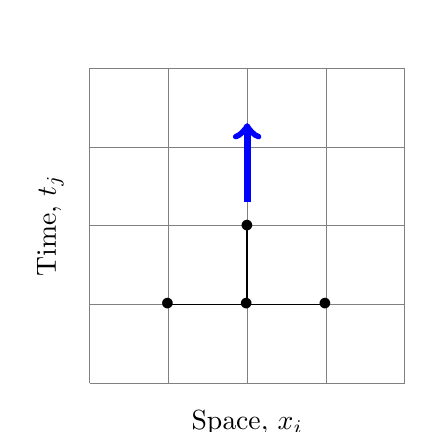
\begin{tikzpicture}
    % Draw the grid
    \draw[very thin, gray] (0,0) grid (4,4);

    % Label the axes
    \node at (2,-0.5) {Space, $x_i$};
    \node[rotate=90] at (-0.5, 2) {Time, $t_j$};

    \foreach \x in {1,2,3} {
        \node at (\x-0.012, 1) {$\bullet$};
    }

    \foreach \x in {1,2} [
        \draw[-, line width=0.05em, black] (\x, 1) -- (\x+1, 1);
    ]

    \draw[-, line width=0.05em, black] (2, 1) -- (2, 2);

    \draw[->, line width=0.25em, blue] (2, 2.3) -- (2, 3.3);
    \node at (2,2-0.012) {$\bullet$}; % Only one point in time step 2 (k=2)
    \end{tikzpicture}
    \caption{Explicit method for the heat equation}
    \label{fig:heat-explicit}
\end{figure}

This is what is known as the explicit scheme.

\subsubsection{Black-Scholes equation}
Similar to the heat equation, the Black Scholes-equation can be discretized to a finite grid of points. For this instance, the domain is defined by time $t \in [0, T]$ (where T represents the expiration time of an option) and asset price $S \in [0,S_{max}]$ (where $S_{max}$ is a sufficiently large upper limit for the underlying asset price). This can be represented by a mesh grid of points.
The time interval $t \in [0, T]$ is divided into $M$ equal-sized time steps, each of size ${\Delta t} = \frac{T}{M}$. Similarly, the asset price range $S \in [0,S_{max}]$ is divided into $N$ equal-sized asset steps, each of size ${\Delta S} = \frac{S_{max}}{N}$.

The price of the option at the current time step will be denoted by $V_i^k$, where $i$ refers to the index representing the asset price grid point  
and $k$ refers to the index representing the time step.

From this, it can be said that the grid points are made up of:
\[
S_i = i {\Delta S},\, t_k = T - k {\Delta t},
\]
where
\[
0 \leq i \leq N \quad \text{and} \quad 0 \leq k \leq M.
\]

Like, in the previous section, the grid can be used to compute an approximation of the option price at the subsequent time step using known values from the current time step. The Black-Scholes equation represents a \textit{backwards} parabolic equation which implies that the subsequent option prices are computed starting from the time at expiration ($t = T$). 

For simplicity, the Black-Scholes equation can be rewritten as such:
\[
\frac{\partial V}{\partial t} + a(S,t) \frac{\partial^2 V}{\partial S^2} + b(S,t) \frac{\partial V}{\partial S} - c(S,t) V = 0
\]
Finite difference approximations will be used to substitute the derivatives of the Black-Scholes PDE:
\begin{align}
\frac{\partial V}{\partial t} &\approx \frac{V_i^k - V_i^{k+1}}{\Delta t} \tag{Theta} \label{eq: theta} \\
\frac{\partial V}{\partial S} &\approx \frac{V_{i+1}^k - V_{i-1}^k}{2 \Delta S} \tag{Delta} \label{eq: delta}\\
\frac{\partial^2 V}{\partial S^2} &\approx \frac{V_{i+1}^k - 2V_i^k + V_{i-1}^k}{\Delta S^2} \tag{Gamma}\label{eq: gamma}
\end{align}
Substituting these three approximations, \eqref{eq: theta}, \eqref{eq: delta}, and \eqref{eq: gamma} into the equation gives us the following:
\[
\frac{V_i^k - V_i^{k+1}}{\Delta t} + a(S,t) \frac{V_{i+1}^k - 2V_i^k + V_{i-1}^k}{(\Delta S)^2} + b(S,t) \frac{V_{i+1}^k - V_{i-1}^k}{2 \Delta S} - c(S,t) V_i^k = 0
\]
The equation is then rearranged such that the $k+1$ terms and $k$ terms are separated:
\[
V_i^{k+1} = A_i^k V_{i-1}^k + (1-B_i^k) V_i^k + C_i^k V_{i+1}^k
\]
{\color{red}What is O?}
where
\begin{align*}
    A_i^k &= a_i^k v_1 - \frac{1}{2} b_i^k v_2 \\
    B_i^k &= -2a_i^k v_1 + c_i^k \Delta t \\
    C_i^k &= a_i^k v_1 + \frac{1}{2} b_i^k v_2 \\
    v_1 &= \frac{\Delta t}{(\Delta S)^2}, \quad v_2 = \frac{\Delta t}{\Delta S}
\end{align*}
The $O(\Delta t^2, \Delta t (\Delta S)^2)$ notation represents the local truncation error.
{\color{red}SO WHAT????!!!! What is the meaning of \textbf{local}?}

The grid below illustrates how the option price at the subsequent time step can be calculated using the neighbouring grid points.


\begin{figure}[H]
    \centering
    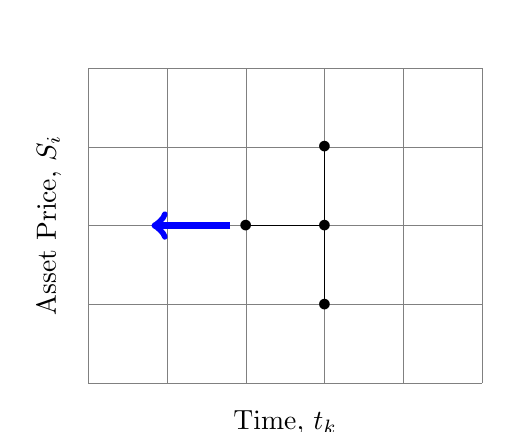
\begin{tikzpicture}
    % Draw the grid
    \draw[very thin, gray] (0,0) grid (5,4);

    % Label the axes
    \node at (2.5,-0.5) {Time, $t_k$};
    \node[rotate=90] at (-0.5, 2) {Asset Price, $S_i$};

    \foreach \y in {1,2,3} {
        \node at (3, \y-0.012) {$\bullet$};
    }
    
    \foreach \y in {1, 2} {
        \draw[-, line width=0.05em, black] (3, \y) -- (3, \y+1);
    }

    \draw[-, line width=0.05em, black] (2, 2) -- (3, 2);

    \draw[->, line width=0.25em, blue] (1.8, 2) -- (0.8, 2);
    \node at (2,2-0.012) {$\bullet$}; 
    \end{tikzpicture}
    \caption{Explicit method for the Black-Scholes equation}
    \label{fig:bse-explicit}
\end{figure}

\subsection{Implicit Scheme: Crank-Nicolson Method}
Despite its straightforward implementation, the explicit method tends to be less stable, as it only takes the current time steps into account for computation. The Crank-Nicolson method addresses this problem by using a combination of the current and subsequent time steps, making it unconditionally stable. It is not confined to the same stability constraints that the explicit method faces.

\subsubsection{Heat equation}
The Crank-Nicolson method involves the approximation of the derivatives at the midpoint of the current and subsequent time steps. By averaging the spatial
second derivatives of both time steps, the following equation is obtained:
\begin{equation}
    \frac{u_i^{j+1} - u_i^j}{\Delta t} = \frac{1}{2(\Delta t)^2} (u_{i+1}^{j+1} - 2u_i^{j+1} + u_{i-1}^{j+1} + u_{i+1}^j - 2u_i^j + u_{i-1}^j),
\end{equation}
which can be rearranged to give
\begin{equation}
    u_i^{j+1} = u_i^j + \frac{\Delta t}{2(\Delta t)^2} (u_{i+1}^{j+1} - 2u_i^{j+1} + u_{i-1}^{j+1} + u_{i+1}^j - 2u_i^j + u_{i-1}^j).
\end{equation}
The equation can be further rewritten to separate the $j+1$ and $j$ terms:
\begin{equation}
    -r u_{i-1}^{j+1} + (1 + 2r) u_i^{j+1} - r u_{i+1}^{j+1} = r u_{i-1}^j + (1 - 2r) u_i^j + r u_{i+1}^j,
\end{equation}
where $r = \frac{\Delta t}{2(\Delta x)^2}$. This leaves us with a tridiagonal system of equations that can be solved to obtain the temperature at the next time step $u_i^{j+1}$.

\begin{figure}[H]
    \centering
    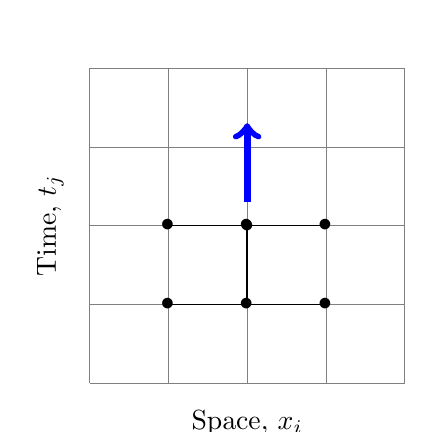
\begin{tikzpicture}
    % Draw the grid
    \draw[very thin, gray] (0,0) grid (4,4);

    % Label the axes
    \node at (2,-0.5) {Space, $x_i$};
    \node[rotate=90] at (-0.5, 2) {Time, $t_j$};

    \foreach \x in {1,2,3} {
        \node at (\x-0.012, 1) {$\bullet$};
        \node at (\x-0.012, 2) {$\bullet$};
    }

    \foreach \y in {1, 2} {
        \draw[-, line width=0.05em, black] (1, \y) -- (3, \y); % Horizontal lines
    }

    \draw[-, line width=0.05em, black] (2, 1) -- (2, 2);

    \draw[->, line width=0.25em, blue] (2, 2.3) -- (2, 3.3);
    \node at (2,2-0.012) {$\bullet$}; % Only one point in time step 2 (k=2)
    \end{tikzpicture}
    \caption{Crank-Nicolson method for the heat equation}
    \label{fig:heat-cn}
\end{figure}


\subsubsection{Black-Scholes equation}
% this needs to be fixed because i use the other way 
Similarly, the Crank-Nicolson method can be applied to the Black-Scholes equation. The equation is rewritten as 
\begin{equation}
    \frac{V_i^{k+1} - V_i^k}{\Delta t} = \frac{1}{2} \left( \mathcal{L}(V_i^{k+1}) + \mathcal{L}(V_i^k) \right)
\end{equation}
such that $\mathcal{L}$ refers to discretized form of the operator that describes how the option value changes. Recall that the following approximations are used for discretization:
\begin{align}
    \frac{\partial V}{\partial t} &\approx \frac{V_i^k - V_i^{k+1}}{\Delta t} \tag{Theta} \\
    \frac{\partial V}{\partial S} &\approx \frac{V_{i+1}^k - V_{i-1}^k}{2 \Delta S} \tag{Delta} \\
    \frac{\partial^2 V}{\partial S^2} &\approx \frac{V_{i+1}^k - 2V_i^k + V_{i-1}^k}{(\Delta S)^2} \tag{Gamma}
 \end{align}
Combine the Explicit (forward) and Implicit (backward) schemes: 
\[
\begin{aligned}
    &\frac{V_i^n - V_i^{n+1}}{\Delta t} + \frac{a_i^{k+1}}{2} \left( \frac{V_{i+1}^{k+1} - 2 V_i^{k+1} + V_{i-1}^{k+1}}{(\Delta S)^2} \right) + \frac{b_i^{k+1}}{2} \left( \frac{V_{i+1}^{k+1} - V_{i-1}^{k+1}}{2 \Delta S} \right) + \frac{1}{2} c_i^{k+1} V_i^{k+1} \\
    &+ \frac{a_i^{k}}{2} \left( \frac{V_{i+1}^{k} - 2 V_i^{k} + V_{i-1}^{k}}{(\Delta S)^2} \right) + \frac{b_i^{k}}{2} \left( \frac{V_{i+1}^{k} - V_{i-1}^{k}}{2 \Delta S} \right) + \frac{1}{2} c_i^{k} V_i^{k} = 0
\end{aligned}
\]
Remove the denominators and rearrange the equation such that the $k+1$ and $k$ terms are separated:
\[
    A_i^{k+1} V_{i-1}^{k+1} + (1+B_i^{k+1})V_i^{k+1} + C_i^{k+1} V_{i+1}^{k+1} = -A_i^k V_{i-1}^{k} + (1-B_i^{k})V_i^{k} + C_i^{k} V_{i+1}^k
\]
where
\begin{align*}
    &A_i^k = \frac{b_i^k v_2}{4} - \frac{a_i^k v_1}{2} \\
    &B_i^k = a_i^k v_1 - \frac{c_i^k}{2} \Delta t \\
    &C_i^k = - \frac{a_i^k v_1}{2} -\frac{b_i^k v_2}{4} \\
    &v_1 = \frac{\Delta t}{(\Delta S)^2}, \quad v_2 = \frac{\Delta t}{\Delta S}
\end{align*}

This is a linear system of equations written in the matrix form of:
\[
    AV^{k+1} = BV^{k}
\]
where $A$ and $B$ represent tridiagonal matrices, and $V^{k+1}$ and $V^{k}$ are vectors containing the option values at the next and current time steps. It is important to note that this is used to solve the interior grid points and only applies to $1 \leq i \leq N_s - 1$, as the boundary conditions address the remaining equations. $N_s$ here refers to the total number of spatial grid points.

This system of equations can be solved to obtain the option values at the next time step $V^{k+1}$.

{\color{red} a few notes about the errors (local/global)?}

\begin{figure}[H]
    \centering
    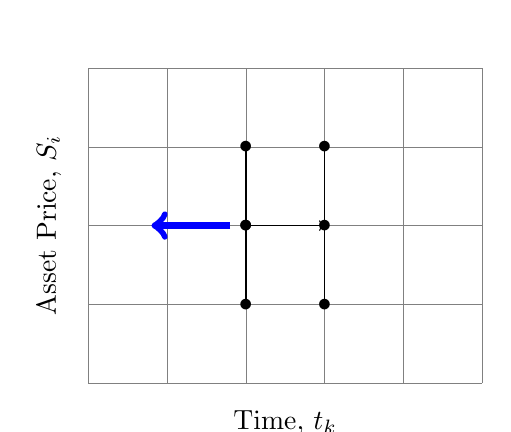
\begin{tikzpicture}
    % Draw the grid
    \draw[very thin, gray] (0,0) grid (5,4);

    % Label the axes
    \node at (2.5,-0.5) {Time, $t_k$};
    \node[rotate=90] at (-0.5, 2) {Asset Price, $S_i$};

    \foreach \y in {1,2,3} {
        \node at (3, \y-0.012) {$\bullet$};
        \node at (2, \y-0.012) {$\bullet$};
    }
    
    \foreach \y in {1, 2} {
        \draw[-, line width=0.05em, black] (2, \y) -- (2, \y+1);
        \draw[-, line width=0.05em, black] (3, \y) -- (3, \y+1);
    }

    \draw[->, line width=0.05em, black] (2, 2) -- (3, 2);
    \draw[->, line width=0.25em, blue] (1.8, 2) -- (0.8, 2);

    \node at (2,2-0.012) {$\bullet$}; 
    \end{tikzpicture}
    \caption{Crank-Nicolson method for the Black-Scholes equation}
    \label{fig:bse-cn}
\end{figure}


\section{Stochastic differential equations}
\subsection{Brownian motion}
\subsection{Ito processes}
\subsection{Geometric Brownian motion}
\subsection{GBM for option pricing}


   
\chapter{Software}\label{sec:software}
% HERE: we just present:
% 1. What the SW does (not how)
% 2. What guarntees the user has that it works (tests), incl. CI
% 3. The fact that it is easy to use
% 4. Convince the reader that the SW is professionally made (e.g., good docs) 
%
% Requirements (what do we want the SW to do)
% SW structure (Python code, classes, CUDA, etc)
%   L  Mini code snippets (not CODE!), e.g., via diagrams
%   L  Link to GH repo
% GitHub Actions (explain what tests)
%   L  Code coverage (?)
%   L  WHAT is being tested? 
%   L  Unit test: boundary/initial conditions
% Other information:
%   L  Licence


\section{Purpose of the Software}
\label{sec:software_purpose}
The software developed in this project provides a Python package of numerical solvers for solving partial differential equations, with a focus on the Black-Scholes equation (BSE).
The current state of the software supports the implementation of finite difference methods, including the explicit and Crank-Nicolson schemes, as well as Monte Carlo simulations for option pricing.
To enhance computational efficiency, the software has been extended to leverage GPU acceleration via CUDA, optimising performance for computationally intensive tasks. 

\section{Software Structure} \label{sec:software_structure}

\subsection{High-Level Architecture}
The software is structured into two main libraries: the Python-based solvers and the GPU-accelerated CUDA C++ solvers. Each component is designed to implement the numerical methods discussed in Section \ref{sec:theory_and_background}. These include:
\begin{itemize}
    \item \textbf{PDESolvers:} This Python library implements finite-difference methods, particularly \textit{explicit} and \textit{Crank-Nicolson}, for solving partial differential equations. Initially designed for the heat and Black-Scholes equation, it has since been extended to focus on the application of the Black-Scholes model on option pricing, including the implementation of Monte Carlo simulations for numerical approximations and analytical solutions for exact pricing. Additionally, the library integrates real market data using the \textit{yfinance} package, allowing key financial metrics such as \textit{volatility} and \textit{mean} to be calculated from historical time-series data. 
    \item \textbf{GPUSolver:} The GPU-accelerated library is designed to optimise the performance of the numerical methods implemented in the PDESolvers library by leveraging GPU parallelisation. These solvers take advantage of the CUDA architecture to accelerate the computationally-intensive parts of the calculation, resulting in significant speed-ups compared to the CPU-based implementation of the same methods.
\end{itemize}


\clearpage 
\begin{landscape}
    \begin{figure}[H]
        \centering
        \begin{landscape}
\begin{figure}[H]
    \centering
\begin{tikzpicture}[scale=0.46, transform shape]

        \begin{umlpackage}[x=-9, y=8]{pdes}
            \umlclass[y=-11]{BlackScholesEquation}{
            - option\_type: OptionType \\
            - S\_max: float \\
            - K: float \\
            - r: float \\
            - sigma: float \\
            - expiry: float \\
            - s\_nodes: int \\
            - t\_nodes: int \\
            - V: np.ndarray 
            }{
                \umlstatic{+ generate\_grid(value: float, nodes: int)} \\
                + s\_nodes: int \{property\} \\
                + t\_nodes: int \{property\} \\
                + option\_type: OptionType \{property\} \\
                + S\_max: float \{property\} \\
                + sigma: float \{property\} \\
                + expiry: float \{property\} \\
                + rate: float \{property\} \\
                + strike\_price: float \{property\}
            }

            \umlclass[y=0]{HeatEquation}{
                - length: float \\
                - x\_nodes: int \\
                - time: float \\
                - t\_nodes: int \\
                - k: float \\
                - initial\_temp: callable \\
                - left\_boundary\_temp: callable \\
                - right\_boundary\_temp: callable
            }{
                + set\_initial\_temp(u0: callable) \\
                + set\_left\_boundary\_temp(left: callable) \\
                + set\_right\_boundary\_temp(right: callable) \\
                + generate\_grid(value: float, nodes: int) \\
                + length: float \{property\} \\
                + time: float \{property\} \\
                + x\_nodes: int \{property\} \\
                + t\_nodes: int \{property\} \\
                + k: float \{property\} \\
                + get\_initial\_temp(x: float): float \\
                + get\_left\_boundary(t: float): float \\
                + get\_right\_boundary(t: float): float
            }
        \end{umlpackage}

        \begin{umlpackage}[x=1, y=12]{solvers}
            \umlclass[x=0, y=0]{BlackScholesExplicitSolver}{
                - equation : BlackScholesEquation
            }{
                + solve()
            }
            
            \umlclass[x=6.5, y=0]{BlackScholesCNSolver}{
                - equation: BlackScholesEquation
            }{
                + solve()
            }

            \umlclass[x=12.3, y=0]{Heat1DExplicitSolver}{
                - equation : HeatEquation
            }{
                + solve()
            }

            \umlclass[x=17.5, y=0]{Heat1DCNSolver}{
                - equation : HeatEquation
            }{
                + solve()
            }

            \umlclass[type=abstract, x=2, y=-4]{Solver}{

            }{
                + solve()
            }

            \umlinherit[geometry=-|]{BlackScholesExplicitSolver}{Solver}
            \umlinherit[geometry=|-]{BlackScholesCNSolver}{Solver}
            \umlinherit[geometry=|-]{Heat1DExplicitSolver}{Solver}
            \umlinherit[geometry=|-]{Heat1DCNSolver}{Solver}

        \end{umlpackage}

        \begin{umlpackage}[x=3, y=1]{solution}
            \umlclass[y=-0.5]{Solution}{
                - result: numpy.array \\
                - x\_grid: numpy.array \\
                - y\_grid: numpy.array \\
                - dx: float \\
                - dy: float \\
                - duration: float 
            }{
                + plot() \\ 
                + get\_result() \\ 
                + get\_execution\_time() \\
                + \_\_sub\_\_(other: Solution) \\
                \# set\_plot\_labels(ax)
            }

            \umlclass[x=6, y=2]{Solution1D}{
                
            }{\# set\_plot\_labels(ax)}

            \umlclass[x=8, y=-3]{SolutionBlackScholes}{
                - option\_type: OptionType \\
                - delta: float \\
                - gamma: float \\
                - theta: float \\
            }{
                + plot\_greek(greek\_type: Greeks, time\_step=int) \\
                \# set\_plot\_labels(ax)
            }

            \umlinherit[geometry=|-]{Solution1D}{Solution}
            \umlinherit[geometry=|-]{SolutionBlackScholes}{Solution}
        \end{umlpackage}

        \begin{umlpackage}[x=-10, y=-12.5]{enums}
            \umlenum{OptionType}{
                EUROPEAN\_CALL \\
                EUROPEAN\_PUT
            }{}

            \umlenum[x=4]{Greeks}{
                DELTA \\
                GAMMA \\
                THETA
            }{}
        \end{umlpackage}

        \begin{umlpackage}[x=26, y=2]{utils}

            \umlclass{Heat1DHelper}{
            }{
                \umlstatic{\# build\_tridiagonal\_matrix(a: float, b: float, c: float, nodes: int)}
            }

            \umlclass[y=-3]{BlackScholesHelper}{
            }{
                \umlstatic{\# calculate\_greeks\_at\_boundary(equation, delta, gamma, theta, tau, V, S, ds)} \\
                \umlstatic{\# set\_boundary\_conditions(equation, T, tau)}
            }

            \umlclass[y=-8]{RBFInterpolator}{
                - z: np.ndarray \\
                - hx: float \\
                - hy: float \\
                - nx: int \\
                - ny: int
            }{
                - get\_coordinates(x: float, y: float) \\
                - euclidean\_distances(x\_minus: float, y\_minus: float, x: float, y: float) \\
                - \umlstatic{rbf(d: float, gamma: float)} \\
                + interpolate(x: float, y: float)
            }

            \umlclass[y=-13.5]{GPUResults}{
                - file\_path: str \\
                - s\_max: float \\
                - expiry: float \\
                - grid\_data: np.ndarray
            }{
                + get\_results()\\
                + plot\_option\_surface()
            }
            
        \end{umlpackage}

        \begin{umlpackage}[x=4, y=-12]{optionspricing}
            \umlclass[x=0,y=-4]{BlackScholesFormula}{
                - option\_type: OptionType \\
                - S0: float \\
                - strike\_price: float \\
                - r: float \\
                - sigma: float \\
                - expiry: float
            }{
                + get\_black\_scholes\_merton\_price()
            }

            \umlclass[x=9,y=0]{MonteCarloPricing}{
                - option\_type: OptionType \\
                - S0: float \\
                - strike\_price: float \\
                - r: float \\
                - sigma: float \\
                - T: float
                - time\_steps: float \\
                - sim: int \\
                - S: np.ndarray \\
                - run: bool
                - duration: float
            }{  
                - generate\_grid() \\
                + simulate\_gbm() \\
                + get\_monte\_carlo\_option\_price() \\
                + get\_execution\_time() \\
                + plot()
            }

            \umlclass[x=0,y=2]{HistoricalStockData}{
                - stock\_data: pd.DataFrame \\
                - ticker: str 
            }{
                + fetch\_stock\_data(start\_date: str, end\_date: str) \\
                + estimate\_metrics() \\
                + get\_latest\_stock\_price() 
            }

        \end{umlpackage}

        \umlcompo{Solver}{Solution}
        \umlassoc[geometry=|-]{MonteCarloPricing}{OptionType}
        \umlassoc{BlackScholesFormula}{OptionType}
        \umlassoc{BlackScholesEquation}{OptionType}
        \umlassoc{SolutionBlackScholes}{OptionType}
        \umlassoc{SolutionBlackScholes}{Greeks}
        \umldep{BlackScholesExplicitSolver}{BlackScholesEquation}
        \umldep{BlackScholesCNSolver}{BlackScholesEquation}
        \umldep{Heat1DExplicitSolver}{HeatEquation}
        \umldep{Heat1DCNSolver}{HeatEquation}
        \umldep{BlackScholesExplicitSolver}{BlackScholesHelper}
        \umldep{BlackScholesCNSolver}{BlackScholesHelper}
        \umldep{Heat1DCNSolver}{Heat1DHelper}

\end{tikzpicture}
\end{figure}
\end{landscape}
        \caption{UML Class Diagram of the \textbf{pdesolvers} Python library}
        \label{fig:uml_class}
    \end{figure}
\end{landscape}
\clearpage

\section{Testing and Reliability} \label{sec:software_testing}
The software has undergone comprehensive testing to verify its correctness and functionality. These tests include checks for boundary conditions, initial conditions and performance benchmarks to ensure that the numerical methods produce accurate and reliable results. To streamline the development process, a CI/CD pipeline has been established using GitHub Actions. This automated pipeline runs tests whenever any changes are pushed to the main branch, ensuring that new feature additions or modifications do not introduce bugs or errors to the software. Code coverage is also monitored to ensure that the tests do not miss any critical parts of the code, providing confidence in the reliability of the software.

For Quality Assurance (QA), pull requests and code reviews were conducted throughout the development of the software. This process involved peer reviews of the code changes, ensuring that the code adheres to best practices and do not break existing functionality.

\subsection{Testing Details}
The testing framework used in this project is \textit{pytest}, which is a widely-used testing framework for Python. The tests are designed to cover various aspects of the software, including:
\begin{itemize}
    \item \textbf{Unit Tests:} These tests validate individual components of the software, ensuring that each function and method behaves as expected. Specifically, they verify that the boundary and initial conditions of the numerical methods are correctly implemented, checking that appropriate constraints are applied throughout the calculations. The tests also include validation for incorrect or unsupported inputs, raising appropriate exceptions to prevent runtime errors.
    \item \textbf{Integration Tests:} Integration tests check the interaction between multiple components of the software to ensure they work correctly. For this instance, the tests focused on comparing the results of different solvers, verifying the approximated solutions against their analytical counterparts, and simulating specific behaviour via mock data. These were particularly done by testing the convergence of the numerical methods from the absolute differences of the approximated solutions or interpolated solutions. Additionally, the Monte Carlo simulations were validated by using mocked data to simulate specific scenarios, ensuring that the simulation produced expected results. 
\end{itemize}


% HERE: we just present:
% 1. What the SW does (not how)
% 2. What guarntees the user has that it works (tests), incl. CI
% 3. The fact that it is easy to use
% 4. Convince the reader that the SW is professionally made (e.g., good docs) 
%
% Requirements (what do we want the SW to do)
% SW structure (Python code, classes, CUDA, etc)
%   L  Mini code snippets (not CODE!), e.g., via diagrams
%   L  Link to GH repo
% GitHub Actions (explain what tests)
%   L  Code coverage (?)
%   L  WHAT is being tested? 
%   L  Unit test: boundary/initial conditions
% Other information:
%   L  Licence


\chapter{Simulations}\label{sec:simulations}
% Alt. title: R E S U L T S
% The idea is that you have used the software to solve many problems
% and you're presenting the results...
%
% 1. Heat equation
% 2. BSE with different solvers (say you got the same solutions)
% 3. Speed-up with GPU solver
%      L  Dolan-Moré plot
% 4. Geom. Br. Motion results (plots)

\section{Heat Equation}\label{sec:heat_equation-results}
For the heat equation, we define the parameters as follows: \textbf{(Length of domain $L = 1$, Spatial nodes $N_x = 100$, Time $= 30$, Time Nodes $N_t = 10000$, Thermal Diffusivity $\kappa = 0.01$)}. It is further combined with the \textbf{initial condition} $u_0(x) = \sin(\pi x) + 5$, with \textbf{time-dependent boundary conditions}: $u(0,t) = 5 \sin\left(\frac{2 \pi}{25} t \right) + 5$ and $u(L,t) = t+5$.

\begin{figure}[H]
    \centering
    \begin{subfigure}[t]{0.45\textwidth}
        \centering
        \includegraphics[width=\textwidth]{figures/heat_explicit.pdf}
        \caption{\textbf{Explicit:} 3D Surface Plot for Heat Equation}
        \label{fig:heat-explicit-3d}
    \end{subfigure}
    \hfill
    \begin{subfigure}[t]{0.45\textwidth}
        \centering
        \includegraphics[width=\textwidth]{figures/heat_cn.pdf}
        \caption{\textbf{Crank-Nicolson:} 3D Surface Plot for Heat Equation}
        \label{fig:heat-cn-3d}
    \end{subfigure}
    \label{fig:heat-3d}
\end{figure}

Figures \ref{fig:heat-explicit-3d} and \ref{fig:heat-cn-3d} visualise the numerical solutions to the defined heat equation using the \textit{explicit} and \textit{Crank-Nicolson} methods respectively. The left boundary introduces a periodic boundary condition which manifests as oscillations observed in both plots at $x=0$. Meanwhile, the right boundary condition leads to a linear increase in temperature over time, as reflected in the steadily rising temperature at $x=1$. Under unfavourable conditions, the explicit method can lead to numerical instability shown in Figure \ref{fig:heat-explicit-unstable}.

\begin{figure}[H]
    \centering
    \includegraphics[width=0.5\textwidth]{figures/heat_explicit_unstable.pdf}
    \caption{\textbf{Explicit:} 3D Surface Plot for Heat Equation ($N_x = 100$, $N_t = 100$)}
    \label{fig:heat-explicit-unstable}
\end{figure}

\section{Black-Scholes Equation}\label{sec:bs_equation-results}
Defining a common set of parameters for the Black-Scholes equation, the implemented solvers (\textit{numerical methods}) are tested against each other to verify their accuracy. The parameters used for the tests are as follows:
\textbf{(Initial Stock Price $S_0 = 300$, Strike Price $K = 100$, Risk-free Rate $r = 0.05$, Volatility $\sigma = 0.2$, Expiry $T = 1$, Spatial Nodes $N_s = 100$, Time Nodes  $N_t = 1000$)}

At a glance, the results of the numerical solvers appear to be displaying similar plots, staying consistent with theoretical expectations. The surface plots for both option types exhibits the expected behaviour, where call option prices stay close to zero when the underlying asset price is significantly below the strike price, particularly as time approaches maturity. The reverse occurs for a put option where the prices are close to zero when the underlying asset price is significantly above the strike price. Call option prices start to rise only when the underlying asset price exceeds the strike price, while put option prices increase when the asset price falls below the strike price.

Similar to Figure \ref{fig:heat-explicit-unstable}, the \textit{explicit} method for the Black-Scholes method can also lead to numerical instability if the time and spatial nodes are not appropriately chosen (shown in Figure \ref{fig:bs-explicit-unstable}). Using the same parameters that led the \textit{explicit} method to be unstable, the \textit{Crank-Nicolson} method remains stable, as seen in Figure \ref{fig:bs-cn-stable}.

\begin{figure}[H]
    \centering
    \begin{subfigure}[t]{0.45\textwidth}
        \centering
        \includegraphics[width=\textwidth]{figures/call_option_explicit.pdf}
        \caption{\textbf{Explicit:} 3D Surface Plot for Call Option}
        \label{fig:bs-explicit-call}
    \end{subfigure}
    \hfill
    \begin{subfigure}[t]{0.45\textwidth}
        \centering
        \includegraphics[width=\textwidth]{figures/call_option_cn.pdf}
        \caption{\textbf{Crank-Nicolson:} 3D Surface Plot for Call Option}
        \label{fig:bs-cn-call}
    \end{subfigure}
    \hfill
    \begin{subfigure}[t]{0.45\textwidth}
        \centering
        \includegraphics[width=\textwidth]{figures/put_option_explicit.pdf}
        \caption{\textbf{Explicit:} 3D Surface Plot for Put Option}
        \label{fig:bs-explicit-put}
    \end{subfigure}
    \hfill
    \begin{subfigure}[t]{0.45\textwidth}
        \centering
        \includegraphics[width=\textwidth]{figures/put_option_cn.pdf}
        \caption{\textbf{Crank-Nicolson:} 3D Surface Plot for Put Option}
        \label{fig:bs-cn-put}
    \end{subfigure}
    \begin{subfigure}[t]{0.45\textwidth}
        \centering
        \includegraphics[width=\textwidth]{figures/bse_unstable.pdf}
        \caption{\raggedright \textbf{Explicit:} 3D Surface Plot for Black-Scholes Equation ($N_s$ = 100, $N_t$ = 100)}
        \label{fig:bs-explicit-unstable}
    \end{subfigure}
    \hfill
    \begin{subfigure}[t]{0.45\textwidth}
        \centering
        \includegraphics[width=\textwidth]{figures/bse_stable.pdf}
        \caption{\raggedright \textbf{Crank-Nicolson:} 3D Surface Plot for Black-Scholes Equation ($N_s = 100$, $N_t$ = 100)}
        \label{fig:bs-cn-stable}
    \end{subfigure}
    \label{fig:bs-3d}
\end{figure}

% At time $t=0$ (i.e. at the initial time step), the option price show a slight curvature before increasing, which is expected as it takes into account the dis

% \begin{figure}[H]
%     \centering
%     \begin{subfigure}[t]{0.45\textwidth}
%         \centering
%         \includegraphics[width=\textwidth]{figures/put_option_explicit.pdf}
%         \caption{\textbf{Explicit:} 3D Surface Plot for Put Option}
%         \label{fig:bs-explicit-put}
%     \end{subfigure}
%     \hfill
%     \begin{subfigure}[t]{0.45\textwidth}
%         \centering
%         \includegraphics[width=\textwidth]{figures/put_option_cn.pdf}
%         \caption{\textbf{Crank-Nicolson:} 3D Surface Plot for Put Option}
%         \label{fig:bs-cn-put}
%     \end{subfigure}
% \end{figure}


\section{GPU Speed-up Analysis}\label{sec:speedup_analysis}
The speed-up achieved by the GPU implementations of the numerical methods was evaluated by comparing their execution times to their corresponding CPU counterparts. The formula for speed-up is given by:
\begin{equation}
    \text{Speedup} = \frac{\text{CPU Execution Time}}{\text{GPU Execution Time}}
\end{equation}
\begin{figure}[H]
    \centering
    \begin{tikzpicture}
        \begin{loglogaxis}[
            xlabel={Spatial Nodes},
            ylabel={Speedup},
            title={Log-Log Plot of Speedup vs s nodes},
            grid=both,
            mark size=2pt,
            legend style={
                at={(1.05,1)},
                anchor=north west
            },
            legend cell align={left}
        ]
        \addplot[
            color=blue,
            mark=*,
        ]
        table[
            x={s nodes},
            y={Speedup},
            col sep=comma
        ] {csv/bse_cn_large_params.csv};
        \addlegendentry{Crank-Nicolson}

        \addplot[
            color=purple,
            mark=square*,
        ]
        table[
            x={s nodes},
            y={Speedup},
            col sep=comma
        ] {csv/bse_explicit_large_params.csv};
        \addlegendentry{Explicit}

        \end{loglogaxis}
    \end{tikzpicture}
    \caption{Speedup vs Spatial Nodes}
    \label{fig:speedup-bse}
\end{figure}

Figure \ref{fig:speedup-bse} presents a log-log plot of speed-up against an increasing number of spatial nodes for the {Crank-Nicolson} and {explicit} methods. The results align with expectations, demonstrating a notable performance speedup with the GPU implementation, especially for larger problem sizes. With smaller problem sizes, particularly with the \textit{Crank-Nicolson} method, the GPU implementation did not yield substantial speed-up where, in some cases, performed slower than the CPU. This is likely due to the GPU being underutilised for smaller cases, where its parallel processing capabilities are not fully leveraged. The plots demonstrate that there is a gradual increase in speed-up initially. However, as the problem size increases, the plot becomes steeper, indicating that the GPU is being utilised more effectively.

Looking at the results, the \textit{explicit} method shows a higher speed-up compared to the \textit{Crank-Nicolson} method, which is expected due to its lower computational complexity. The latter method requires a more complex solution process that involves solving a system of linear equations per time step, which can be more computationally intensive.

\section{Geometric Brownian Motion and Monte Carlo Simulations}\label{sec:gbm_results}

For reproducibility, a seed has been set for the random number generator, ensuring that the results can be replicated. The following parameters will be used to obtain the results for the Geometric Brownian Motion (GBM) and Monte Carlo simulations: 
\textbf{(Initial Stock Price $S_0 = 300$, Strike Price $K = 100$, Risk-free Rate $r = 0.05$, Volatility $\sigma = 0.2$, Expiry $T = 1$, Time Steps $\tau = 365$, Simulations = $1000$, Seed $= 78$)}

Figures \ref{fig:price-distribution-lower-vol} and \ref{fig:price-distribution-higher-vol} show the distribution of underying asset prices at expiry for two different volatility levels ($\sigma = 0.2$ and $\sigma = 0.4$). The distribution of prices at expiry is expected to be log-normally distributed, as the GBM model assumes that the logarithm of the asset prices follows a normal distribution. The figures illustrate this behaviour, with the distribution becoming wider as the volatility increases.

\begin{figure}[H]
    \centering
    \begin{subfigure}[t]{0.45\textwidth}
        \centering
        \includegraphics[width=\textwidth]{figures/monte_carlo_prices_small_vol.pdf}
        \caption{Distribution of prices ($\sigma=0.2$)}
        \label{fig:price-distribution-lower-vol}
    \end{subfigure}
    \hfill
    \begin{subfigure}[t]{0.45\textwidth}
        \centering
        \includegraphics[width=\textwidth]{figures/monte_carlo_prices_high_vol.pdf}
        \caption{Distribution of prices ($\sigma=0.4$)}
        \label{fig:price-distribution-higher-vol}
    \end{subfigure}
    \caption{Distribution of Asset Prices at Expiry}
    \label{fig:price-distribution}
\end{figure}

The distribution of payoffs at expiry is shown in Figures \ref{fig:payoff-distribution-call} and \ref{fig:payoff-distribution-put}. 

\begin{figure}[H]
    \centering
    \begin{subfigure}[t]{0.45\textwidth}
        \centering
        \includegraphics[width=\textwidth]{figures/monte_carlo_payoff_call.pdf}
        \caption{Distribution of payoff for Call Option ($K = 100, \sigma = 0.2$)}
        \label{fig:payoff-distribution-call}
    \end{subfigure}
    \hfill
    \begin{subfigure}[t]{0.45\textwidth}
        \centering
        \includegraphics[width=\textwidth]{figures/monte_carlo_payoff_put.pdf}
        \caption{Distribution of payoff for Put Option ($K = 600, \sigma = 0.2$)}
        \label{fig:payoff-distribution-put}
    \end{subfigure}
    \caption{Distribution of Payoff at Expiry}
    \label{fig:payoff-distribution}
\end{figure}

The effect of increasing the number of simulations on the accuracy of the Monte Carlo simulation is illustrated in Figure \ref{fig:convergence}. Despite some discrepancies, a general downward trend in the absolute error is observed as the number of simulations increase, indicating that the prices eventually converge towards the analytical solution which is expected due to the law of large numbers.
\begin{figure}[H]
    \centering
    \begin{tikzpicture}
        \begin{loglogaxis}[
            xlabel={Number of Simulations},
            ylabel={Absolute Error},
            title={Absolute Error vs Number of Simulations},
            grid=both,
            mark size=2pt,
            legend style={
                at={(1.05,1)},
                anchor=north west
            },
            legend cell align={left}
        ]
        \addplot[
            color=blue,
            mark=*,
        ]
        table[
            x={Simulations},
            y={Error},
            col sep=comma
        ] {csv/benchmark_errors.csv};

        \end{loglogaxis}
    \end{tikzpicture}
    \caption{Absolute Error vs Number of Simulations}
    \label{fig:convergence}
\end{figure}

\section{Comparison of Numerical Methods}\label{sec:comparison_numerical_methods}
Using the same parameters from the previous sections, the results of each numerical method can be compared against each other to validate the accuracy of the solvers. The table of results in \ref{tab:comparison-explicit-cn} shows the absolute error between the \textit{explicit} and \textit{Crank-Nicolson} methods over a range of dimensions. 


\textbf{(Option Type: Call, Initial Stock Price $S_0 = 300$, Strike Price $K = 100$, Risk-free Rate $r = 0.05$, Volatility $\sigma = 0.2$, Expiry $T = 1$)}

\begin{table}[H]
    \centering
    \begin{tabular}
        { |c|c|c| }
        \hline
        \textbf{$N_s$} & \textbf{$N_t$} & \textbf{Absolute Error between Explicit and Crank-Nicolson (3 s.f.)} \\ \hline
            10 & 100 & 0.00451 \\ \hline
            50 & 1000 & 0.00279 \\ \hline
            100 & 1000 & 0.00502 \\ \hline
            100 & 10000 & 0.000498 \\ \hline
            100 & 50000 & 0.0000996 \\ \hline
            1000 & 50000 & 0.00105 \\ \hline
            1000 & 100000 & 0.000520 \\ \hline
    \end{tabular}
    \caption{Absolute Error between Explicit and Crank-Nicolson}
    \label{tab:comparison-explicit-cn}
\end{table}

Looking at these results, the absolute error between the two solvers appears to converge towards zero as the grid dimensions become increasingly fine. This behaviour suggests that both methods are consistent with one another and validates the correctness of the numerical methods used. However, this increase in accuracy comes with a trade-off in terms of computational time due to the increasing number of calculations required. As mentioned earlier in Section \ref{sec:speedup_analysis}, the \textit{Crank-Nicolson} method is expected to be more computationally expensive than the \textit{explicit} method due to the additional calculations required to solve the system of linear equations. 

% To address this computational cost, the GPU-accelerated implementations of the solvers were introduced to offload the most computationally intensive operations to the GPU. 
Here, we compare the GPU-accelerated solvers against their CPU counterparts to evaluate the correctness of the GPU implementations. The results of the absolute error between the GPU and CPU implementations are shown in Table \ref{tab:comparison-cpu-gpu}.

\begin{table}[H]
    \centering
    \begin{minipage}{0.48\textwidth}
        \centering
        \begin{tabular}{ |c|c|c| }
            \hline
            \textbf{$N_s$} & \textbf{$N_t$} & \textbf{Abs. Error (3 s.f.)} \\ \hline
            101 & 1001 & 0.000500 \\ \hline
            101 & 10001 & 0.000500 \\ \hline
            100 & 50000 & 0.000500 \\ \hline
            1001 & 50001 & 0.000500 \\ \hline
        \end{tabular}
        \caption{\textbf{Explicit}}
        \label{tab:comparison-cpu-gpu-explicit}
    \end{minipage}
    \hfill
    \begin{minipage}{0.48\textwidth}
        \centering
        \begin{tabular}{ |c|c|c| }
            \hline
            \textbf{$N_s$} & \textbf{$N_t$} & \textbf{Abs. Error (3 s.f.)} \\ \hline
            101 & 1001 & 0.000500 \\ \hline
            101 & 10001 & 0.000500 \\ \hline
            101 & 50001 & 0.000500 \\ \hline
            1001 & 50001 & 0.000500 \\ \hline
        \end{tabular}
        \caption{\textbf{Crank-Nicolson}}
        \label{tab:comparison-cpu-gpu-cn}
    \end{minipage}
    \caption{Absolute Error between CPU and GPU}
    \label{tab:comparison-cpu-gpu}
\end{table}

These results show that the absolute error between the CPU and GPU implementations is consistently low, indicating that the GPU implementations are producing results that are consistent with their CPU counterparts. This suggests that the parallelised computations on the GPU do not compromise the accuracy of the numerical results despite the increased computational speed. This consistency validates the correctness of the GPU-accelerated solvers and confirms that the integrity of the numerical methods is preserved.

\subsubsection{Accuracy of Interpolated Solutions}

Additionally, the accuracy of the interpolated solutions was evaluated by comparing the maximum absolute differences (errors) of the coarse and fine grid solutions as shown in Table \ref{tab:interpolation-error}.

\begin{table}[H]
    \centering
    \begin{minipage}{0.48\textwidth}
        \centering
        \begin{tabular}{|c|c|c|}
            \hline
            \textbf{Coarse} & \textbf{Fine} & \makecell{\textbf{Max Abs.}\\\textbf{Error (5 s.f.)}} \\
            \hline
            $101 \times 1001$ & $101 \times 2001$ & 0.021715 \\ \hline
            $101 \times 1001$ & $201 \times 4001$ & 0.51812 \\ \hline
            $101 \times 8001$ & $301 \times 4001$ & 0.063388 \\ \hline
            $201 \times 4001$ & $101 \times 10001$ & 0.50181 \\ \hline
            $101 \times 4001$ & $201 \times 10001$ & 0.50452 \\ \hline
        \end{tabular}
        \subcaption{\textbf{Explicit}}
        \label{tab:interpolation-explicit}
    \end{minipage}
    \hfill
    \begin{minipage}{0.48\textwidth}
        \centering
        \begin{tabular}{|c|c|c|}
            \hline
            \textbf{Coarse} & \textbf{Fine} & \makecell{\textbf{Max Abs.}\\\textbf{Error (5 s.f.)}} \\
            \hline
            $101 \times 1001$ & $101 \times 2001$ & 0.021707 \\ \hline
            $101 \times 1001$ & $201 \times 4001$ & 0.51794 \\ \hline
            $101 \times 8001$ & $301 \times 4001$ & 0.062640 \\ \hline
            $201 \times 4001$ & $101 \times 10001$ & 0.50181 \\ \hline
            $101 \times 4001$ & $201 \times 10001$ & 0.50452 \\ \hline
        \end{tabular}
        \subcaption{\textbf{Crank-Nicolson}}
        \label{tab:interpolation-cn}
    \end{minipage}
    \caption{Absolute error between interpolated coarse and fine grid solutions.}
    \label{tab:interpolation-error}
\end{table}

\subsubsection{Testing against Analytical Solution}
As a standard benchmark, the solvers were tested against the analytical solution of the Black-Scholes equation to further validate the accuracy of the numerical methods. 

\begin{table}[H]
    \centering
    \caption{Model Parameters for Numerical Experiments}
    \label{tab:model-parameters}
    \begin{tabular}{lccc}
        \toprule
        \textbf{Parameter} & \textbf{Symbol} & \textbf{Finite Difference Methods} & \textbf{Monte Carlo} \\
        \midrule
        Initial Stock Price & $S_0$ & 300 & 300 \\
        Strike Price & $K$ & 100 & 100 \\
        Risk-free Rate & $r$ & 0.05 & 0.05 \\
        Volatility & $\sigma$ & 0.2 & 0.2 \\
        Expiry & $T$ & 1 & 1 \\
        Spatial Nodes & $N_s$ & 100 & -- \\
        Time Nodes & $N_t$ & 2000 & -- \\
        Time Steps & $\tau$ & -- & 365 \\
        Number of Simulations & -- & -- & 100,000 \\
        Random Seed & -- & -- & 42 \\
        \bottomrule
    \end{tabular}
\end{table}

\begin{table}[H]
    \centering
    \begin{tabular}
        { |c|c|c|c| }
        \hline
        \textbf{Analytical Solution} & \textbf{Explicit} & \textbf{Crank-Nicolson} & \textbf{Monte-Carlo Price} \\ \hline
        204.8770575757042 & 204.8770575499286 & 204.8770575499286 & 204.73167692582822\\ \hline
    \end{tabular}
    \caption{Comparison between Analytical and Numerical Solutions}
    \label{tab:comparison-of-option-prices}
\end{table}

Table \ref{tab:comparison-of-option-prices} shows that the \textit{Explicit} and \textit{Crank-Nicolson} methods yield numerical solutions that are approximately close to the analytical solution, differing only at a small magnitude of $2.578 \times 10^{-8}$. This demonstrates the level of accuracy and reliability the finite difference methods can achieve when solving the Black-Scholes equation. Contrastly, the Monte Carlo simulations approximates the option price at a slight deviation of $0.1453806498758$ from the analytical solution. This discrepancy is expected due to the stochastic nature of the Monte Carlo method, which relies on random sampling to estimate the option price. While not as precise as the finite difference methods, the Monte Carlo method remains within an acceptable range to provide a reasonable approximation of the option price. This, however, can only be achieved when using a sufficiently large number of simulations, as shown in Figure \ref{fig:convergence}. 



% Alt. title: R E S U L T S
% The idea is that you have used the software to solve many problems
% and you're presenting the results...
%
% 1. Heat equation
% 2. BSE with different solvers (say you got the same solutions)
% 3. Speed-up with GPU solver
%      L  Dolan-Moré plot
% 4. Geom. Br. Motion results (plots)

\chapter{Conclusions}\label{sec:conclusions}
% \chapter{Results \& Discussion}\label{sec:results_and_discussion}
% \input{text/05_results_discussion}
        
% \chapter{Conclusions \& Future Work}\label{sec:conclusions_and_futurework}
% \section{Assessment of achievements}
This project set out to achieve: \textbf{(i)} the design and implementation of a multirotor attitude control system using an \ac{LQR} controller, and an \ac{AHRS} using a 9 \ac{DoF} \ac{IMU} and a \ac{KF} state estimator, and \textbf{(ii)} the design, build and test flight of a viable tilting-wings and tilting-rotors quadrotor.

The specification outcomes of completing those two achievements were that I would:
\begin{enumerate}
    \item have an excellent understanding of how quadcopters work, including certain details about their aerodynamics. \\$\rightarrow$ \textcolor{green!80!black}{Complete}, see Section \ref{sec:aerodynamics}. In particular, I used quaternion-based equations of motion of the quadrotor along with the aerodynamics equations to model the voltage-to-thrust dynamics and the reaction wheel effect.
    \item be able to design control and estimation systems for quadcopters (especially LQR and Kalman filters). \\$\rightarrow$ \textcolor{green!60!black}{Complete}, see Section \ref{sec:control_and_estimation}. Specifically, I studied the theory of linear-quadratic optimal control and optimal estimation for linear systems, and applied it to a linearisation of the model created above; I became familiar with the tuning parameters, usually denoted $Q$ and $R$, of the said control and estimation systems' optimisation problems.
    \item perform simulations of dynamical systems in either MATLAB or Python. \\$\rightarrow$ \textcolor{green!60!black}{Complete}, see Section \ref{sec:simulations}, where I developed a detailed and realistic simulator in Python (part of the Deadcopter library).
    \item have developed strong embedded programming skills. \\$\rightarrow$ \textcolor{green!60!black}{Complete}, see Section \ref{sec:software}, where I implemented the above control and estimation systems in a header-only Arduino library, which is C++ (but implemented more as C with classes). This involved creating classes, polling input pins, extensive debugging, and investigating the limits of the Arduino Due in terms of modifying interrupt service routine priorities.
    \item have become familiar with LiPo battery charging. \\$\rightarrow$ \textcolor{green!60!black}{Complete}, see Section \ref{sec:lipo_battery}. In particular, the methods and benefits of keeping a battery healthy, and the potentially destructive dangers of overcharging.
    \item be able to operate a small drone using an appropriate radio controller and be able to integrate different systems involving hardware and software components. \\
    $\rightarrow${} 
    \textcolor{green!60!black}{Complete (not tested)}, see Section \ref{sec:limitations_and_further_developments} and Specification Objectives 4, 5 and 6 in Section \ref{sec:progress_review}. This involved extensive integration of hardware components, and just as extensive integration of the hardware components with the software; tasks such as building and printing the wings to fit on the frame, extending the frame legs to accommodate the wings, profiling graphite spars for mounting the motors, integrating the \fnstt{Servo} and \fnstt{DueTimer} libraries to work with my custom-made PPM deciphering function and controlling the ESCs with the \fnstt{Servo} library to name a few. Further work involved tasks such as interpreting data from an IMU and troubleshooting the radio transmitter and receiver with an oscilloscope. If the project was to be repeated, I would choose to spend more of the budget on a reliable and robust controller, and a receiver with a serial output.
\end{enumerate}
There were many other outcomes in addition to these, such as learning the quaternion number system, modelling linear \ac{MIMO} dynamical systems, gaining in-depth knowledge of the \ac{PWM} and \ac{PPM} protocols, how to simulate system and measurement noise, general DIY skills, 3D \ac{CAD} and printing skills, using code libraries in Python and C/C++, implementing a code generator using Jinja2, designing and building test benches, managing project progress and software using IT (e.g., Git, issue trackers and pull requests), researching the market, and very importantly, conducting risk assessments. Having gained all of this knowledge and these skills, I will be better informed and more useful in all future projects.








\section{Limitations and further developments}\label{sec:limitations_and_further_developments}
There was one main limitation on this project; space. The lack of a suitably safe lab space for conducting further physical tests meant I was unable to test fly the quadrotor in order to complete testing. At the beginning of the project, I extended the specification to a more ambitious one, which made for an intensive, yet rewarding, year. Given more time and test space, the following tasks would be carried out, in this particular order:
\begin{enumerate}
    \item Create unit and integration tests for Python scripts and generated Arduino code.
    \item Develop code generator to filter multiplications by zero out of the flight controller calculations.
    \item Design and build robust container that bolts onto frame to hold the avionics, servos and battery.
    \item Test fly quadrotor and investigate flight characteristics in both quadcopter and aeroplane mode.
    \item Refactor Deadcopter and release the first version on pypi.org (so that people can install it with: pip install deadcopter).
    \item Implement a black box: a data logger on an on-board SD card.
\end{enumerate}

Additionally, in light of Amazon.com, Inc. winning approval for their ``Prime Air'' drone delivery fleet last year \cite{amazon}, I would investigate the following ideas which are based on increasing payload capability and flight range.
\begin{itemize}
    \item A slingshot-type drone launcher to enable a larger-than-maximum vertical take-off weight payload when launching drone so that wing lift is provided from the start and only very short runways are needed. After payload is delivered, aircraft weight will be reduced so that vertical take-off is possible from the delivery point.
    \item Wing extensions are pulled open before launch to give maximum lift during outbound flight, then springs will pull extensions back in after payload delivery to reduce drag for inbound journey as less lift is required. The springs are actuated by a solenoid after delivery.
\end{itemize}
       


\pagebreak
\bibliographystyle{IEEEtran}
\bibliography{references}

% \pagebreak
% \appendix
% \chapter{Parts List with Cost}\label{app:parts_list}
\begin{table}[htpb!]
    \centering
    \scriptsize
    \begin{tabular}{p{3.5cm}|p{1.5cm}|p{1.5cm}|p{7.5cm}}
        \hline
        \multicolumn{4}{c}{\normalsize{\textbf{Parts List}}}\\
        \hline
        \textbf{Name} & \textbf{Units} & \textbf{Unit Cost (£)} & \textbf{Notes}\\
        \hline
        Battery & $1$ & $36$ & Rhino 4000mAh 4S 50C with XT90 connector\\
        \hline
        Battery Voltmeter & $1$ & $3$ & compatible up to at least 4S\\
        \hline
        Battery Charger & $1$ & $32$ & compatible up to at least 4S\\
        \hline
        Frame & $1$ & $20$ & F450, 282 grams, built-in power distribution board\\
        \hline
        ESC w/UBEC & $4$ & $11$ & 4S compatible, with Universal Battery Eliminating Circuit (5V, 5A)\\
        \hline
        Brushless Motor & $4$ & $13$ & Turnigy 3730 1000kV\\
        \hline
        Motor Spar & $2$ & $8$ & igus 10mm graphite rod modified to mount motors\\
        \hline
        Motor Spar Mount & $4$ & $1$ & two pairs, 3D printed\\
        \hline
        Propeller & $12$ & $1.5$ & 8",9",10", two pairs, clockwise and counter clockwise\\
        \hline
        Foam Wing & $1$ & $30$ & made from strong lightweight foam\\
        \hline
        Wing Extension & $2$ & $3$ & 3D printed, slides inside foam wing\\
        \hline
        Wing Spar & $1$ & $15$ & igus 10mm graphite rod\\
        \hline
        Pillow Bearing & $2$ & $3$ & igus 10mm, for holding wing spar\\
        \hline
        Threaded Bar & $1$ & $20$ & nylon, M10, for legs\\
        \hline
        Arduino Due & $1$ & $40$ & 7-12 \si{\volt} input, 3.3 \si{\volt} logic, regulated outputs of 3.3 and 5 \si{\volt}\\
        \hline
        LLC & $1$ & $2.5$ & bi-directional, between 5 and 3.3 \si{\volt}\\
        \hline
        IMU & $1$ & $8$ & MPU9250\\
        \hline
        Servo & $3$ & $20$ & 25 \si{\kilogram\per\centi\meter} DS Servo with metal gear\\
        \hline
        Buzzer & $1$ & $1$ & 5 \si{\volt} supply, can be actuated with 3.3 \si{\volt}\\
        \hline
        SD Card & $1$ & $6$ & stores flight data\\
        \hline
        SD Card Reader & $1$ & $6$ & writes flight data to SD card, Arduino Due compatible\\
        \hline
        Radio Controller & $1$ & $57$ & Turnigy 9X 2.4 GHz, uses AFHDS 2A protocol\\
        \hline
        Radio Receiver & $1$ & $0$ & Turnigy iA8, uses AFHDS 2A protocol, includes PPM output, bundled with Tx\\
        \hline
        XT90 Connectors & $1$ & $3$ & for connecting battery to distribution board\\
        \hline
        Velcro Tape & $1$ & $5$ & for attaching battery and avionics to frame\\
        \hline
        X Weave Tape & $1$ & $5.5$ & for making foam wings\\
        \hline
        Cable Extensions & $1$ & $9$ & allowing servo placement anywhere on frame\\
        \hline
        Total & & $359.5$ & \\
        \hline
    \end{tabular}
    \label{tab:parts_list}
\end{table}



\end{document}          
